\subsection{Biểu đồ Hoạt động (Activity Diagram)}

Biểu đồ hoạt động mô tả chi tiết các luồng xử lý, các bước thực hiện và các điểm quyết định rẽ nhánh trong một quy trình nghiệp vụ cụ thể. Dưới đây là hai biểu đồ hoạt động cho các chức năng cốt lõi của hệ thống.

\begin{figure}[H]
    \centering
    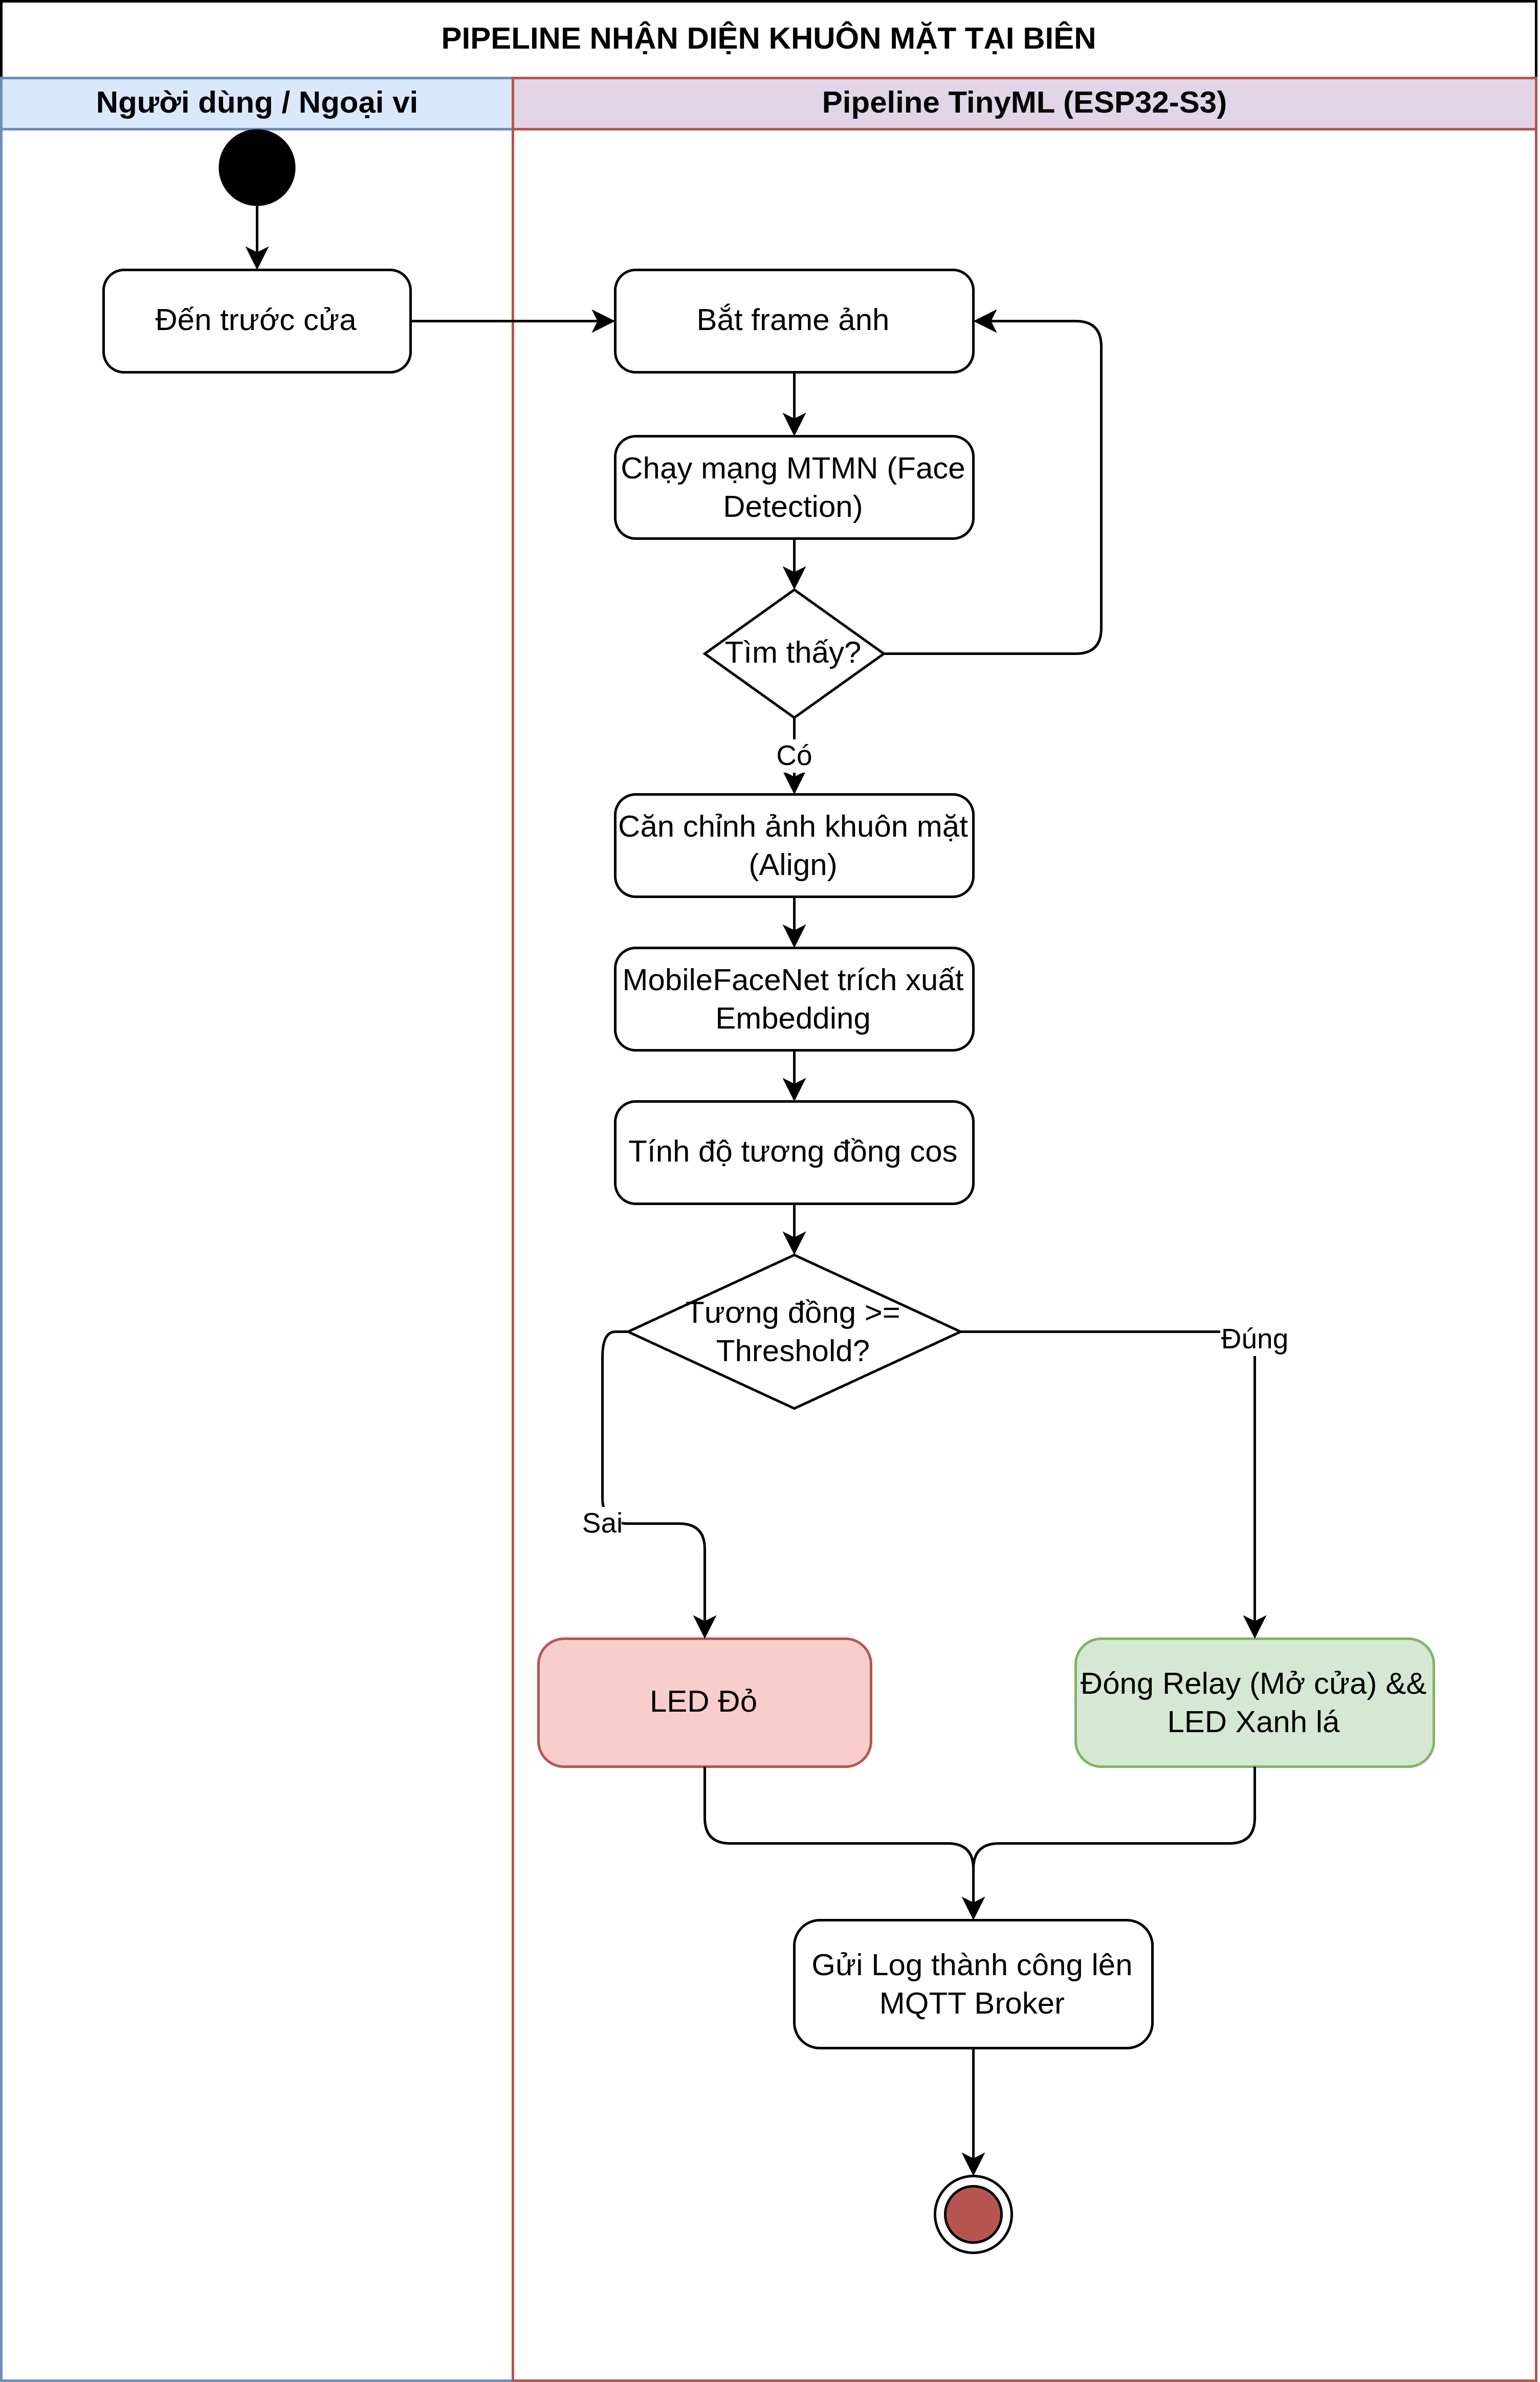
\includegraphics[width=0.8\textwidth]{images/ad-mo khoa.png}
    \caption{Biểu đồ hoạt động cho luồng "Nhận diện khuôn mặt tại biên"}
    \label{fig:ad_mo_khoa}
\end{figure}

\begin{figure}[H]
    \centering
    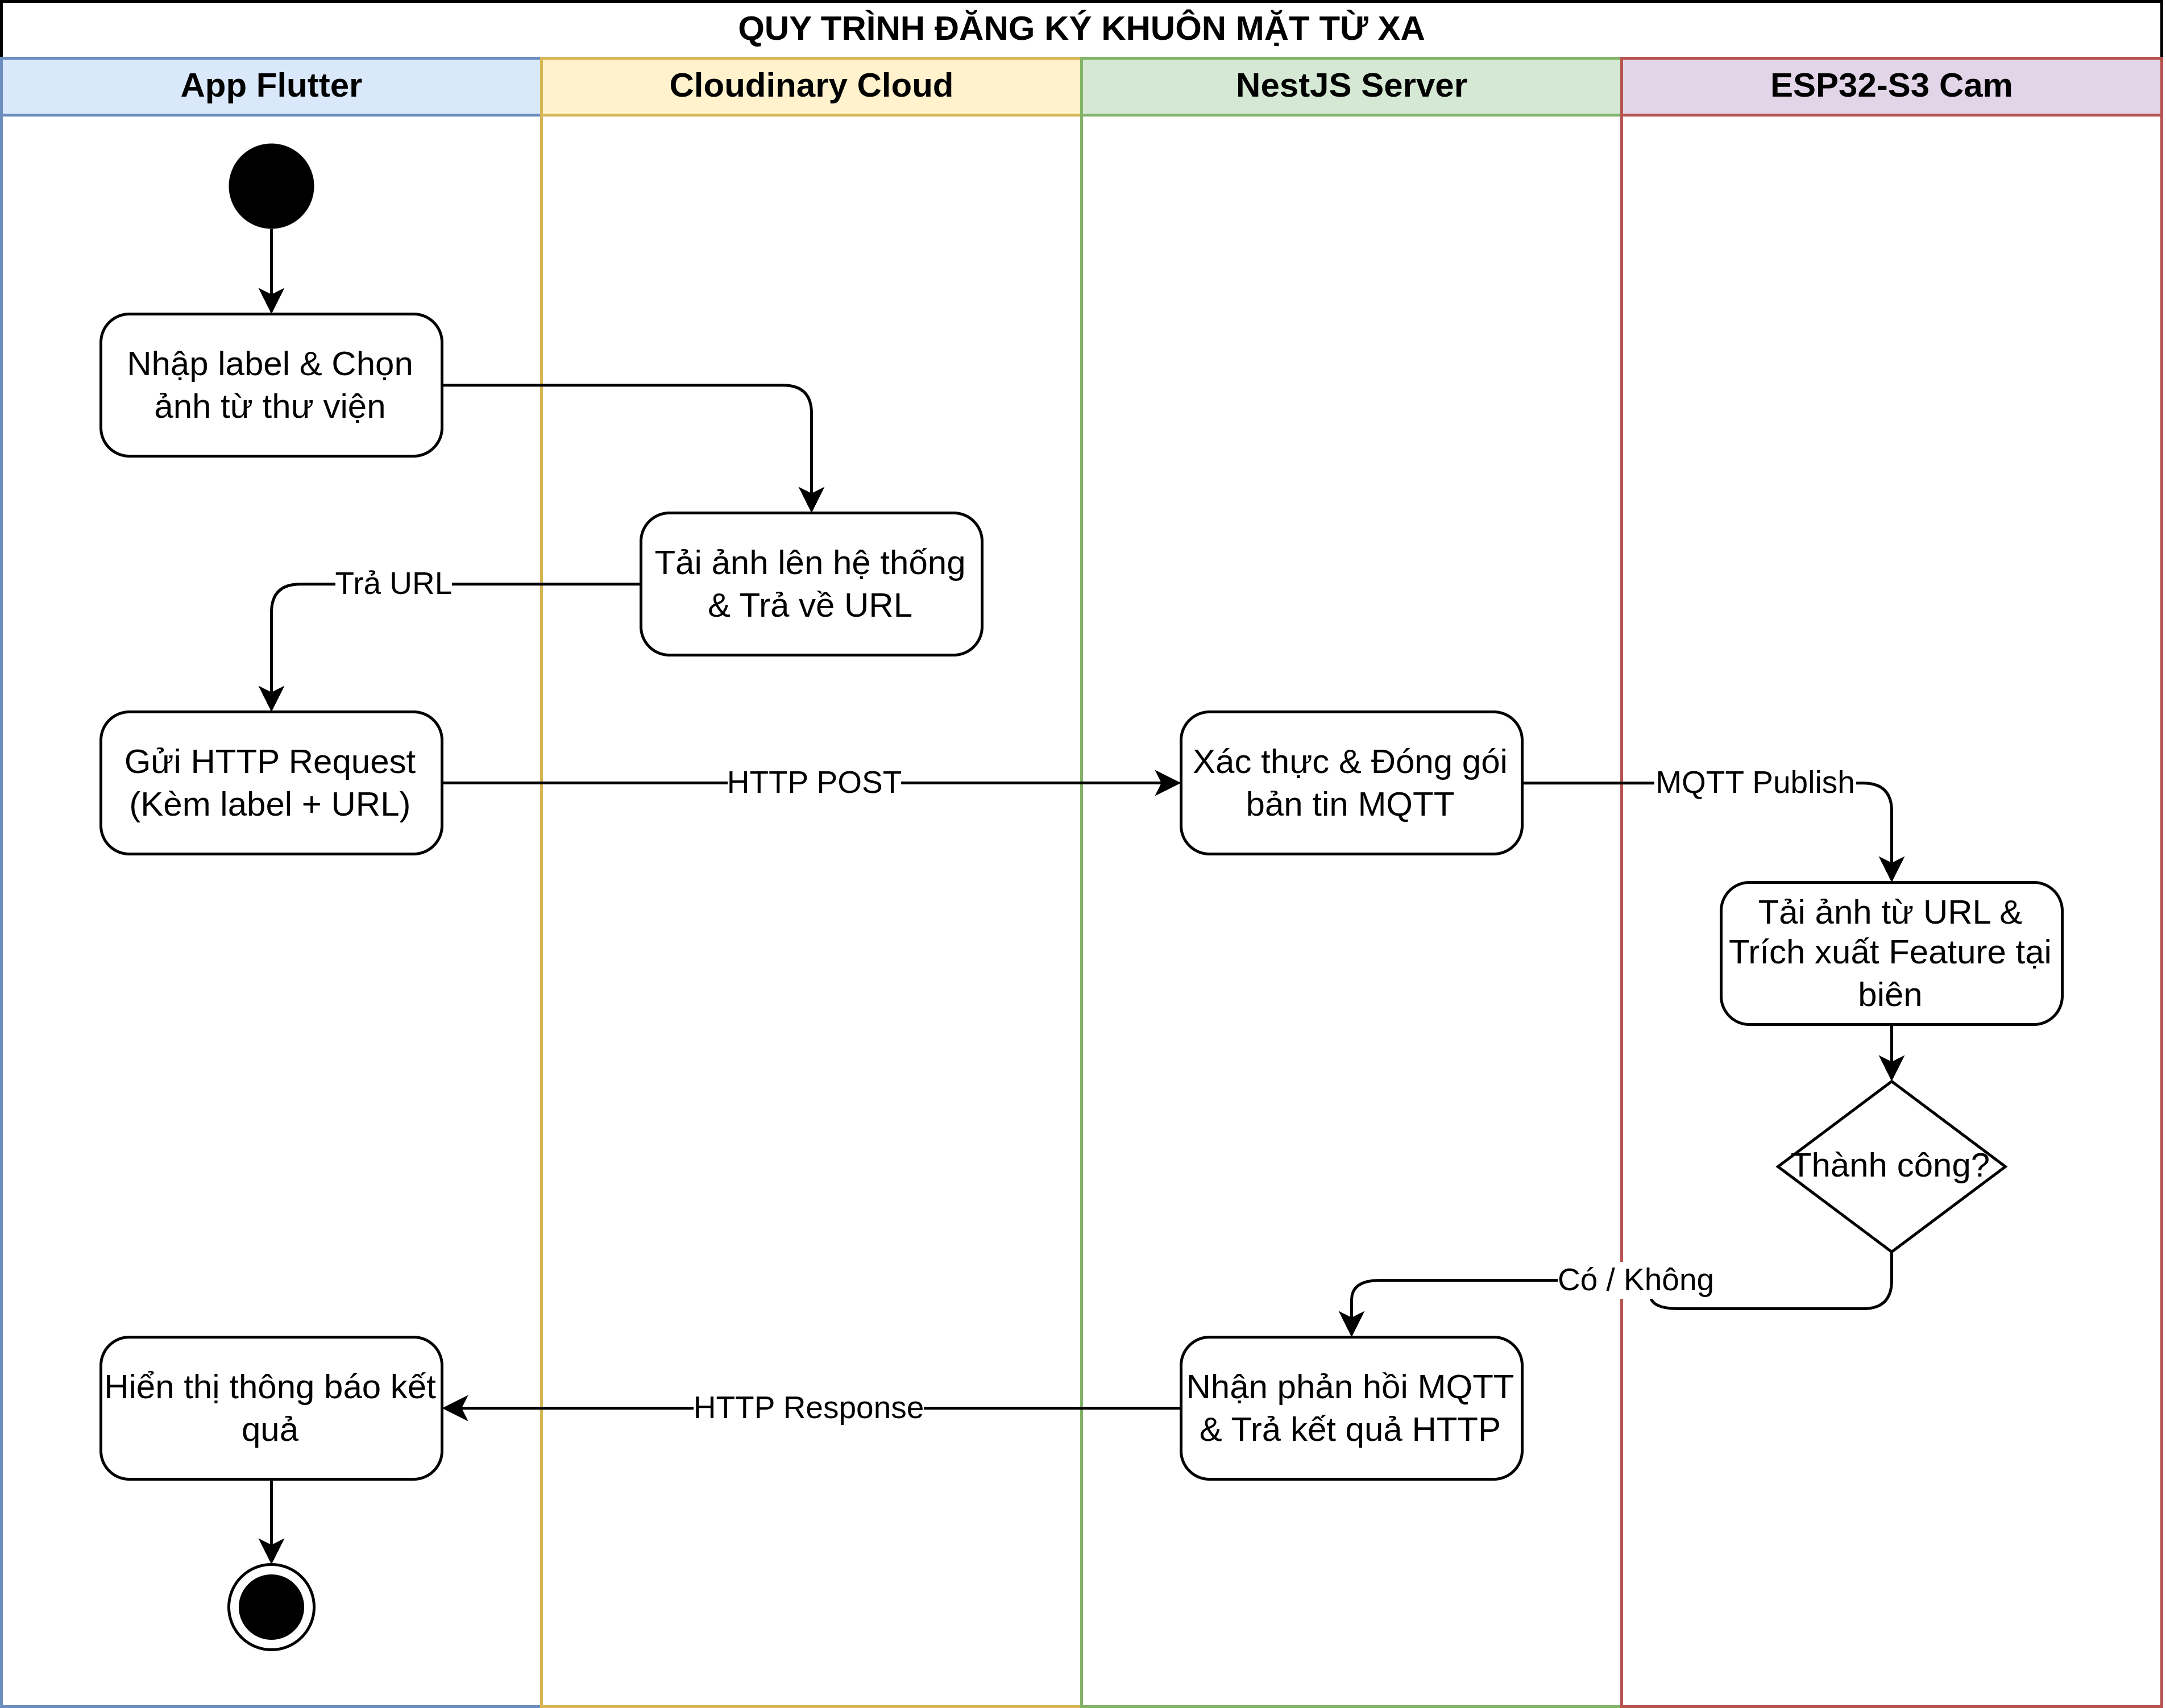
\includegraphics[width=0.8\textwidth]{images/ad-dk mat.png}
    \caption{Biểu đồ hoạt động cho luồng "Đăng ký khuôn mặt mới"}
    \label{fig:ad_dk_mat}
\end{figure}